\chapter{Временные ряды}


\begin{problem}
Что такое автокорреляция?
\end{problem}

\begin{solution}
\end{solution}


\begin{problem}
На графике представлены данные по уровню озера Гур\'{о}н в футах в 1875-1972 годах:  




\begin{knitrout}
\definecolor{shadecolor}{rgb}{0.969, 0.969, 0.969}\color{fgcolor}\begin{kframe}
\begin{alltt}
\hlkwd{ggplot}\hlstd{(df,} \hlkwd{aes}\hlstd{(}\hlkwc{x} \hlstd{= obs,} \hlkwc{y} \hlstd{= level))} \hlopt{+} \hlkwd{geom_line}\hlstd{()} \hlopt{+} \hlkwd{labs}\hlstd{(}\hlkwc{x} \hlstd{=} \hlstr{"\textbackslash{}320\textbackslash{}223\textbackslash{}320\textbackslash{}276\textbackslash{}320\textbackslash{}264"}\hlstd{,}
    \hlkwc{ylab} \hlstd{=} \hlstr{"\textbackslash{}320\textbackslash{}243\textbackslash{}321\textbackslash{}200\textbackslash{}320\textbackslash{}276\textbackslash{}320\textbackslash{}262\textbackslash{}320\textbackslash{}265\textbackslash{}320\textbackslash{}275\textbackslash{}321\textbackslash{}214 \textbackslash{}320\textbackslash{}276\textbackslash{}320\textbackslash{}267\textbackslash{}320\textbackslash{}265\textbackslash{}321\textbackslash{}200\textbackslash{}320\textbackslash{}260 (\textbackslash{}321\textbackslash{}204\textbackslash{}321\textbackslash{}203\textbackslash{}321\textbackslash{}202\textbackslash{}321\textbackslash{}213)"}\hlstd{)}
\end{alltt}
\end{kframe}
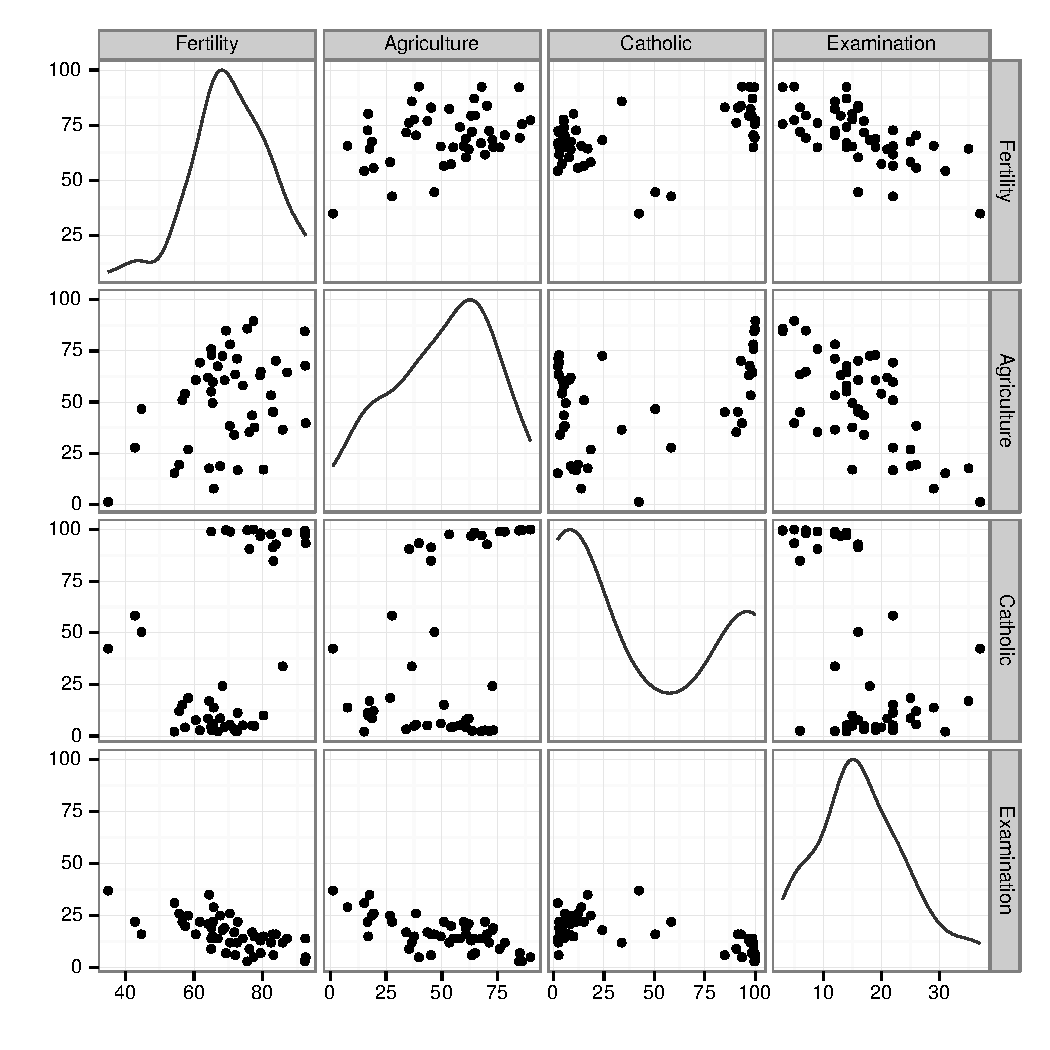
\includegraphics[width=6cm,height=6cm]{figure/unnamed-chunk-2} 

\end{knitrout}


График автокорреляционной и частной автокорреляционной функций:

\begin{knitrout}
\definecolor{shadecolor}{rgb}{0.969, 0.969, 0.969}\color{fgcolor}\begin{kframe}
\begin{alltt}
\hlkwd{ggplot}\hlstd{(acfs.df,} \hlkwd{aes}\hlstd{(}\hlkwc{x} \hlstd{= lag,} \hlkwc{y} \hlstd{= acf,} \hlkwc{fill} \hlstd{= acf.type))} \hlopt{+} \hlkwd{geom_histogram}\hlstd{(}\hlkwc{position} \hlstd{=} \hlstr{"dodge"}\hlstd{,}
    \hlkwc{stat} \hlstd{=} \hlstr{"identity"}\hlstd{)} \hlopt{+} \hlkwd{xlab}\hlstd{(}\hlstr{"\textbackslash{}320\textbackslash{}233\textbackslash{}320\textbackslash{}260\textbackslash{}320\textbackslash{}263"}\hlstd{)} \hlopt{+} \hlkwd{ylab}\hlstd{(}\hlstr{"\textbackslash{}320\textbackslash{}232\textbackslash{}320\textbackslash{}276\textbackslash{}321\textbackslash{}200\textbackslash{}321\textbackslash{}200\textbackslash{}320\textbackslash{}265\textbackslash{}320\textbackslash{}273\textbackslash{}321\textbackslash{}217\textbackslash{}321\textbackslash{}206\textbackslash{}320\textbackslash{}270\textbackslash{}321\textbackslash{}217"}\hlstd{)} \hlopt{+}
    \hlkwd{guides}\hlstd{(}\hlkwc{fill} \hlstd{=} \hlkwd{guide_legend}\hlstd{(}\hlkwc{title} \hlstd{=} \hlkwa{NULL}\hlstd{))} \hlopt{+} \hlkwd{geom_hline}\hlstd{(}\hlkwc{yintercept} \hlstd{=} \hlnum{1.96}\hlopt{/}\hlkwd{sqrt}\hlstd{(}\hlkwd{nrow}\hlstd{(df)))} \hlopt{+}
    \hlkwd{geom_hline}\hlstd{(}\hlkwc{yintercept} \hlstd{=} \hlopt{-}\hlnum{1.96}\hlopt{/}\hlkwd{sqrt}\hlstd{(}\hlkwd{nrow}\hlstd{(df)))}
\end{alltt}
\end{kframe}
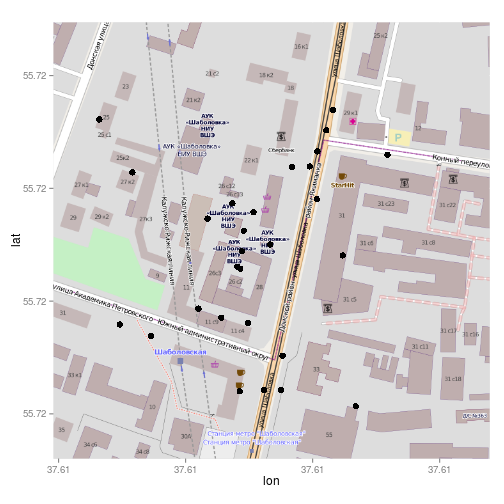
\includegraphics[width=6.5cm,height=6cm]{figure/unnamed-chunk-3} 

\end{knitrout}



\begin{enumerate}
\item Судя по графикам, какие модели класса ARMA или ARIMA имеет смысл оценить?
\item По результатам оценки некоей модели ARMA c двумя параметрами, исследователь посчитал оценки автокорреляционной функции для остатков модели. Известно, что для остатков модели первые три выборочные автокорреляции равны соответственно $0.0047$, $-0.0129$ и $-0.063$. С помощью подходящей статистики проверьте гипотезу о том, что первые три корреляции ошибок модели равны нулю.
\end{enumerate}
\end{problem}

\begin{solution}
\begin{enumerate}
\item Процесс $AR(2)$, т.к. две первые частные корреляции значимо отличаются от нуля, а гипотезы о том, что каждая последующая равна нулю не отвергаются.
\item Можно использовать одну из двух статистик
\[
\text{Ljung-Box}=n(n+2)\sum_{k=1}^3\frac{\hat{\rho}_k^2}{n-k}=
0.4289
\]
\[
\text{Box-Pierce}=n\sum_{k=1}^3\hat{\rho}_k^2=
0.4076
\]
Критическое значение хи-квадрат распределения с 3-мя степенями свободы для $\alpha=0.05$ равно $\chi^2_{3,crit}=7.8147$.
Вывод: гипотеза $H_0$ об отсутствии корреляции ошибок модели не отвергается.
\end{enumerate}
\end{solution}





\begin{problem}
Винни-Пух пытается выявить закономерность в количестве придумываемых им каждый день ворчалок.  Винни-Пух решил разобраться, является ли оно стационарным процессом, для этого он оценил регрессию

\[ \Delta \hat{y}_t = \underset{(0.5)}{4.5} - \underset{(0.1)}{0.4}y_{t-1} +\underset{(0.5)}{0.7} \Delta y_{t-1} \]

Из-за опилок в голове Винни-Пух забыл, какой тест ему нужно провести, то ли Доктора Ватсона, то ли Дикого Фуллера. 

\begin{enumerate}
\item Аккуратно сформулируйте основную и альтернативную гипотезы
\item Проведите подходящий тест на уровне значимости 5\%
\item Сделайте вывод о стационарности ряда
\item Почему Сова не советовала Винни-Пуху пользоваться широко применяемым в Лесу $t$-распределением?
\end{enumerate}
\end{problem}

\begin{solution}




\begin{enumerate}
\item $H_0$: ряд содержит единичный корень, $\beta=0$; $H_0$: ряд не содержит единичного корня, $\beta<0$
\item $ADF=-0.4/0.1=-4$, $ADF_{crit}=-2.89$, $H_0$ отвергается
\item Ряд стационарен
\item При верной $H_0$ ряд не стационарен, и  $t$-статистика имеет не $t$-распределение, а распределение Дики-Фуллера.
\end{enumerate}
\end{solution}



\begin{problem}
Рассматривается модель $y_t=\beta_1+\beta_2 x_{t1}+\ldots+\beta_k x_{tk}+\e_t$. Ошибки $\e_t$ гомоскедастичны, но в них возможно присутствует автокорреляция первого порядка, $\e_t=\rho \e_{t-1}+u_t$. При известном числе наблюдений $T$ на уровне значимости 5\% сделайте статистический вывод о наличии автокорреляции.
\begin{enumerate}
\item $T=25$, $k=2$, $DW=0.8$
\item $T=30$, $k=3$, $DW=1.6$
\item $T=50$, $k=4$, $DW=1.8$
\item $T=100$, $k=5$, $DW=1.1$
\end{enumerate}
\end{problem}

\begin{solution}
\end{solution}


\begin{problem}
По 100 наблюдениям была оценена модель линейной регрессии
$y_t=\beta_1+\beta_2 x_t+\e_t$. Оказалось, что $RSS=120$, $\he_1=-1$, $\he_{100}=2$, $\sum_{t=2}^{100} \he_t\he_{t-1}=-50$. Найдите $DW$ и $\rho$.
\end{problem}

\begin{solution}
\end{solution}


\begin{problem}
Применяется ли статистика Дарбина-Уотсона для выявления автокорреляции в следующих моделях
\begin{enumerate}
\item $y_t=\beta_1 x_t + \e_t$
\item $y_t=\beta_1 + \beta_2 x_t + \e_t$
\item $y_t=\beta_1 + \beta_2 y_{t-1} + \e_t$
\item $y_t=\beta_1 + \beta_2 t +\beta_3 y_{t-1} + \e_t$
\item $y_t=\beta_1 t + \beta_2 x_t + \e_t$
\item $y_t=\beta_1 + \beta_2 t +\beta_3 x_t +\beta_4 x_{t-1} + \e_t$
\end{enumerate}
\end{problem}

\begin{solution}
\end{solution}


\begin{problem}
По 21 наблюдению была оценена модель линейной регрессии
$\underset{(se)}{\hat{y}}=\underset{(0.3)}{1.2}+\underset{(0.18)}{0.9}\cdot y_{t-1}+\underset{(0.01)}{0.1}\cdot t$, $R^2=0.6$, $DW=1.21$. Протестируйте гипотезу об отсутствии автокорреляции ошибок на уровне значимости 5\%.
\end{problem}

\begin{solution}
\end{solution}



\begin{problem}
По 24 наблюдениям была оценена модель линейной регрессии
$\underset{(se)}{\hat{y}}=\underset{(0.01)}{0.5}+\underset{(0.02)}{2}\cdot t$, $R^2=0.9$, $DW=1.3$. Протестируйте гипотезу об отсутствии автокорреляции ошибок на уровне значимости 5\%.
\end{problem}

\begin{solution}
\end{solution}


\begin{problem}
По 32 наблюдениям была оценена модель линейной регрессии
$\underset{(se)}{\hat{y}}=\underset{(2.5)}{10}+\underset{(0.5)}{2.5}\cdot t- \underset{(0.01)}{0.1}\cdot t^2$, $R^2=0.75$, $DW=1.75$. Протестируйте гипотезу об отсутствии автокорреляции ошибок на уровне значимости 5\%.
\end{problem}

\begin{solution}
\end{solution}


\begin{problem}
Рассмотрим модель $y_t=\beta_1+\beta_2 x_{t1}+\ldots+\beta_k x_{tk}+\e_t$, где $\e_t$ подчиняются автокорреляционной схеме первого порядка, т.е.
\begin{enumerate}
\item $\e_t=\rho \e_{t-1}+u_t$, $-1<\rho<1$
\item $\Var(\e_t)=const$, $\E(\e_t)=const$
\item $\Var(u_t)=\sigma^2$, $\E(u_t)=0$
\item Величины $u_t$ независимы между собой
\item Величины $u_t$ и $\e_s$ независимы, если $t\geq s$
\end{enumerate}
Найдите:
\begin{enumerate}
\item $\E(\e_t)$, $\Var(\e_t)$
\item $\Cov(\e_t,\e_{t+h})$
\item $\Corr(\e_t,\e_{t+h})$
\end{enumerate}
\end{problem}

\begin{solution}
\begin{enumerate}
\item $\E(\e_t)=0$, $\Var(\e_t)=\sigma^2/(1-\rho^2)$
\item $\Cov(\e_t,\e_{t+h})=\rho^h\cdot \sigma^2/(1-\rho^2)$
\item $\Corr(\e_t,\e_{t+h})=\rho^h$
\end{enumerate}
\end{solution}



\begin{problem}
Ошибки в модели $y_t=\beta_1+\beta_2 x_{t}+\e_t$ являются автокоррелированными первого порядка, $\e_t=\rho \e_{t-1}+u_t$. Шаман-эконометрист Ойуун выполняет два камлания-преобразования. Поясните смысл камланий:
\begin{enumerate}
\item Камлание А, при $t\geq 2$, Ойуун преобразует уравнение к виду $y_t-\rho y_{t-1}=\beta_1(1-\rho)+ \beta_2(x_t-\rho x_{t-1})+\e_t-\rho \e_{t-1}$
\item Камлание Б, при $t=1$, Ойуун преобразует уравнение к виду $\sqrt{1-\rho^2}y_1=\sqrt{1-\rho^2}\beta_1+\sqrt{1-\rho^2}\beta_2 x_1+\sqrt{1-\rho^2}\e_1$.
\end{enumerate}
\end{problem}

\begin{solution}
\end{solution}


\begin{problem}
Пусть $y_{t}$ --- стационарный процесс. Верно ли, что стационарны: 
\begin{enumerate}
\item $z_{t}=2y_{t}$ 
\item $z_{t}=y_{t}+1$ 
\item $z_{t}=\Delta y_{t}$ 
\item $z_{t}=2y_{t}+3y_{t-1}$ 
\end{enumerate} 
\end{problem}

\begin{solution}
все линейные комбинации стационарны
\end{solution}





\begin{problem}
Известно, что временной ряд $y_{t}$ порожден стационарным процессом, задаваемым соотношением $y_{t}=1+0.5y_{t-1}+\varepsilon_{t}$. Имеется 1000 наблюдений. Вася построил регрессию $y_{t}$ на константу и $y_{t-1}$. Петя построил регрессию на константу и $y_{t+1}$. Какие примерно оценки коэффициентов они получат? 
\end{problem}

\begin{solution}
Они будут примерно одинаковы. Оценка наклона определяется автоковариационной функцией.
\end{solution}



%%%%%%%%%%%%%%%%%% ARCH-GARCH

\begin{problem}
Рассмотрим следующий AR(1)-ARCH(1) процесс, 
$y_{t}=1+0.5y_{t-1}+\varepsilon_{t}$, $\varepsilon_{t}=\nu_{t}\cdot \sigma_{t}$ \\
$\nu_{t}$ независимые $N(0;1)$ величины. \\
$\sigma^{2}_{t}=1+0.8\varepsilon^{2}_{t-1}$\\
Также известно, что $y_{100}=2$, $y_{99}=1.7$ 
\begin{enumerate}
\item Найдите $\E_{100}(\varepsilon^{2}_{101})$, $\E_{100}(\varepsilon^{2}_{102})$, $\E_{100}(\varepsilon^{2}_{103})$, $\E(\varepsilon^{2}_{t})$ 
\item $\Var(y_{t})$, $\Var(y_{t}|\mathcal{F}_{t-1})$ 
\item Постройте доверительный интервал для $y_{101}$:
\begin{enumerate}
\item проигнорировав условную гетероскедастичность 
\item учтя условную гетерескедастичность 
\end{enumerate} 
\end{enumerate} 
\end{problem}

\begin{solution}
\end{solution}


%%%%%%%%%%%%%%%%% Оператор лага

\begin{problem}
Пусть $x_{t}$, $t=0,1,2,...$ - случайный процесс и $y_{t}=(1+\L )^{t}x_{t}$.
Выразите $x_{t}$ с помощью $y_{t}$ и оператора лага $\L $.
\end{problem}

\begin{solution}
$x_{t}=(1-\L )^{t}y_{t}$
\end{solution}


\begin{problem}
Пусть $ F_{n} $ --- последовательность чисел Фибоначчи. Упростите величину
\[ F_{1}+C^{1}_{5}F_{2}+C^{2}_{5}F_{3}+C^{3}_{5}F_{4}+C^{4}_{5}F_{5}+C^{5}_{5}F_{6} \]
\end{problem}

\begin{solution}
$ F_{n}=\L (1+\L )F_{n} $, значит $ F_{n}=\L ^{k}(1+\L )^{k}F_{n} $ или $ F_{n+k}=(1+\L )^{k}F_{n} $
\end{solution}



\begin{problem}
Пусть $y_{t}$, $t=...-2,-1,0,1,2,...$ - случайный процесс. И $y_{t}=x_{-t}$. Являются ли верными рассуждения?
\begin{enumerate}
\item $\L y_{t}=\L x_{-t}=x_{-t-1}$
\item $\L y_{t}=y_{t-1}=x_{-t+1}$ 
\end{enumerate}
\end{problem}

\begin{solution}
а - неверно, б - верно. 
\end{solution}



%%%%%%%%%%%%%%%% состояние-наблюдение, фильтр Калмана


\begin{problem}
Представьте процесс AR(1),
$y_{t}=0.9y_{t-1}-0.2y_{t-2}+\varepsilon_{t}$,
$\varepsilon\sim$WN(0;1) в виде модели состояние-наблюдение. \\
а) Выбрав в качестве состояний вектор $\left(%
\begin{array}{c}
  y_{t} \\
  y_{t-1} \\
\end{array}%
\right)$ \\
б) Выбрав в качестве состояний вектор $\left(%
\begin{array}{c}
  y_{t} \\
  \hat{y}_{t,1} \\
\end{array}%
\right)$ \\
Найдите дисперсии ошибок состояний 
\end{problem}

\begin{solution}
\end{solution}

\begin{problem}
Представьте процесс MA(1),
$y_{t}=\varepsilon_{t}+0.5\varepsilon_{t-1}$,
$\varepsilon\sim$WN(0;1) в виде модели состояние-наблюдение. \\
a) $\left(%
\begin{array}{c}
  \varepsilon_{t} \\
  \varepsilon_{t-1} \\
\end{array}%
\right)$ \\
b) $\left(%
\begin{array}{c}
  \varepsilon_{t}+0.5\varepsilon_{t-1} \\
  0.5\varepsilon_{t} 
\end{array}%
\right)$ 
\end{problem}

\begin{solution}
\end{solution}

\begin{problem}
Представьте процесс ARMA(1,1),
$y_{t}=0.5y_{t-1}+\varepsilon_{t}+\varepsilon_{t-1}$,
$\varepsilon\sim$WN(0;1) в
виде модели состояние-наблюдение. \\
Вектор состояний имеет вид $x_{t},x_{t-1}$, где
$x_{t}=\frac{1}{1-0.5L}\varepsilon_{t}$ 
\end{problem}

\begin{solution}
\end{solution}


\begin{problem}
Рекурсивные коэффициенты 
\begin{enumerate}
\item Oцените модель вида $y_{t}=a+b_{t}x_{t}+\varepsilon_{t}$,
где $b_{t}=b_{t-1}$. 
\item Сравните графики filtered state и smoothed state. 
\item Сравните финальное состояние $b_{T}$ с коэффициентом в
обычной модели линейной регрессии, $y_{t}=a+bx_{t}+\varepsilon_{t}$. 
\end{enumerate}
\end{problem}

\begin{solution}
\end{solution}


\begin{problem}
Пусть $u_t$ --- независимые нормальные случайные величины с 
математическим ожиданием $0$ и дисперсией $\sigma^2$. Известно, что $\e_1=u_1$, $\e_t=u_1+u_2+\ldots+u_t$. Рассмотрим модель $y_t=\beta_1+\beta_2 x_t + \e_t$.

\begin{enumerate}
\item Найдите $\Var(\e_t)$, $\Cov(\e_t,\e_s)$, $\Var(\e)$
\item Являются ли ошибки $\e_t$ гетероскедастичными?
\item Являются ли ошибки $\e_t$ автокоррелированными?
\item Предложите более эффективную оценку вектора коэффициентов регрессии по сравнению МНК-оценкой.
\item Результаты предыдущего пункта подтвердите симуляциями Монте-Карло на компьютере.
\end{enumerate}
\end{problem}

\begin{solution}
\end{solution}


\begin{problem}
Найдите безусловную дисперсию GARCH-процессов 
\begin{enumerate}
\item $\e_t=\sigma_t \cdot \z_t$, $\sigma^2_t=0.1+0.8\sigma^2_{t-1}+0.1\e^2_{t-1}$
\item $\e_t=\sigma_t \cdot \z_t$, $\sigma^2_t=0.4+0.7\sigma^2_{t-1}+0.1\e^2_{t-1}$
\item $\e_t=\sigma_t \cdot \z_t$, $\sigma^2_t=0.2+0.8\sigma^2_{t-1}+0.1\e^2_{t-1}$
\end{enumerate}
\end{problem}

\begin{solution}
$1$, $2$, $2$ 
\end{solution}


\begin{problem}
Являются ли верными следующие утверждения?
\begin{enumerate}
\item GARCH-процесс является процессом белого шума, условная дисперсия которого
изменяется во времени
\item Модель GARCH(1,1) предназначена для прогнозирования меры изменчивости цены
финансового инструмента, а не для прогнозирования самой цены инструмента
\item При помощи GARCH-процесса можно устранять гетероскедастичность
\item Безусловная дисперсия GARCH-процесса изменяется во времени
\item Модель GARCH(1,1) может быть использована для прогнозирования
волатильности финансовых инструментов на несколько торговых недель вперёд     
\end{enumerate}
\end{problem}

\begin{solution}
\end{solution}


\begin{problem}
Рассмотрим GARCH-процесс $\e_t=\sigma_t \cdot \z_t$, $\sigma^2_t=k+g_1\sigma^2_{t-1}+a_1\e^2_{t-1}$. Найдите
\begin{enumerate}
\item $\E(\z_t)$, $\E(\z_t^2)$, $\E(\e_t)$, $\E(\e_t^2)$
\item $\Var(\z_t)$, $\Var(\e_t)$, $\Var(\e_t \mid \mathcal{F}_{t-1})$
\item $\E(\e_t \mid \mathcal{F}_{t-1})$, $\E(\e_t^2 \mid \mathcal{F}_{t-1})$, $\E(\sigma^2_t \mid \mathcal{F}_{t-1})$
\item $\E(\z_t\z_{t-1})$, $\E(\z_t^2\z_{t-1}^2)$, $\Cov(\e_t,\e_{t-1})$, $\Cov(\e_t^2,\e_{t-1}^2)$
\item $\lim_{h\to\infty} \E(\sigma^2_{t+h} \mid \mathcal{F}_t)$
\end{enumerate}
\end{problem}

\begin{solution}
\end{solution}


\begin{problem}
Используя 500 наблюдений дневных логарифмических доходностей $y_t$ ,
была оценена GARCH(1,1)-модель: $\hy_t=-0.000708+\he_t$, $\e_t=\sigma_t \cdot \z_t$, $\sigma^2_t=0.000455+0.6424\sigma^2_{t-1}+0.2509\e^2_{t-1}$. Также известно, что $\hat{\sigma}^2_{499}=0.002568$, $\he^2_{499}=0.000014$, $\he^2_{500}=0.002178$.
Найдите 
\begin{enumerate}
\item  $\hat{\sigma}^2_{500}$, $\hat{\sigma}^2_{501}$, $\hat{\sigma}^2_{502}$
\item Волатильность в годовом выражении в процентах, соответствующую
наблюдению с номером $t = 500$
\end{enumerate}
\end{problem}

\begin{solution}
\end{solution}


\begin{problem}
Докажите, что в условиях автокорреляции МНК-
оценки остаются несмещенными.
\end{problem}

\begin{solution}
\end{solution}


\begin{problem}
Продавец мороженного оценил динамическую модель объёмов продаж:
\[
\ln \hat{Q}_t=26.7 + 0.2\ln \hat{Q}_{t-1}-0.6\ln P_t
\]
Здесь $Q_t$ --- число проданных в день $t$ вафельных стаканчиков, а $P_t$ --- цена одного стаканчика в рублях. Продавец также рассчитал остатки $\hat{e}_t$.
\begin{enumerate}
\item Чему, согласно полученным оценкам, равна долгосрочная эластичность объёма продаж по цене?
\item Предположим, что продавец решил проверить наличие автокорреляции первого порядка с помощью теста Бройша-Годфри. Выпишите уравнение регрессии, которое он должен оценить.  
\end{enumerate}
\end{problem}

\begin{solution}
\end{solution}

\begin{problem}
Рассматривается модель $y_t = \mu + \varepsilon_t$, $t = 1,\ldots,T$, где $\varepsilon_t = \rho \varepsilon_{t-1} + u_t$, случайные величины $\varepsilon_0, u_1,\dots,u_T$ независимы, причем $\varepsilon_0 \sim N(0,\sigma^2/(1 - \rho^2))$, $u_t \sim N(0,\sigma^2)$. Имеются наблюдения $y' = (1, 2, 0, 0, 1)$.
\begin{enumerate}
  \item Выпишите функцию правдоподобия 
  \[
  \mathrm{L}(\mu, \rho, \sigma^2) = f_{Y_1}(y_1)\prod_{t=2}^{T}f_{Y_t|Y_{t-1}}(y_t|y_{t-1}).
  \]
  \item Найдите оценки неизвестных параметров модели максимизируя условную функцию правдоподобия 
  \[
  \mathrm{L}(\mu, \rho, \sigma^2|Y_1 = y_1) = \prod_{t=2}^{T}f_{Y_t|Y_{t-1}}(y_t|y_{t-1})
  \] 
\end{enumerate}
\end{problem}

\begin{solution}
1. Поскольку имеют место соотношения $\varepsilon_1 = \rho \varepsilon_0 + u_1$ и $Y_1 =\mu + \varepsilon_1$, то из условия задачи получаем, что $\varepsilon_1 \sim N(0,\sigma^2 / (1 - \rho^2))$
и $Y_1 \sim N(\mu,\sigma^2 / (1 - \rho^2))$. Поэтому
\[
f_{Y_1}(y_1) = \frac{1}{\sqrt{2\pi\sigma^2/(1-\rho^2)}}\exp{\left(-\frac{(y_1 - \mu)^2}{2\sigma^2/(1 - \rho^2)}\right)}.
\]

Далее, найдем $f_{Y_2|Y_1}(y_2|y_1)$. Учитывая, что $Y_2 = \rho Y_1 + (1- \rho) \mu + u_2$, получаем $Y_2|\{Y_1 = y_1\} \sim N(\rho y_1 + (1- \rho) \mu, \sigma^2)$. Значит,
\[
f_{Y_2|Y_1}(y_2|y_1) = \frac{1}{\sqrt{2\pi\sigma^2}}\exp{\left(-\frac{(y_2 - \rho y_1 - (1- \rho) \mu)^2}{2\sigma^2}\right)}.
\]

Действуя аналогично, получаем, что для всех $t \geq 2$ справедлива формула
\[
f_{Y_{t}|Y_{t-1}}(y_{t}|y_{t-1}) = \frac{1}{\sqrt{2\pi\sigma^2}}\exp{\left(-\frac{(y_{t} - \rho y_{t-1} - (1- \rho) \mu)^2}{2\sigma^2}\right)}.
\]

Таким образом, находим функцию правдоподобия
\[
\mathrm{L}(\mu, \rho, \sigma^2) = f_{Y_T,\ldots,Y_1}(y_T,\dots,y_1) = f_{Y_1}(y_1)\prod_{t=2}^{T}f_{Y_t|Y_{t-1}}(y_t|y_{t-1}) \text{,}
\]
где $f_{Y_1}(y_1)$ и $f_{Y_t|Y_{t-1}}(y_t|y_{t-1})$ получены выше.

2. Для нахождения неизвестных параметров модели запишем логарифмическую условную функцию правдоподобия:
\[
l(\mu, \rho, \sigma^2|Y_1 = y_1) = \sum_{t=2}^{T}\log{f_{Y_t|Y_{t-1}}(y_t|y_{t-1})} = 
\]
\[
=-\frac{T-1}{2} \log(2 \pi) - \frac{T-1}{2} \log{\sigma^2} - \frac{1}{2\sigma^2} \sum_{t=2}^{T}(y_t - \rho y_{t-1} - (1 - \rho) \mu)^2 \text{.} 
\]

Найдем производные функции $l(\mu, \rho, \sigma^2|Y_1 = y_1)$ по неизвестным параметрам:
\[
\frac{\partial l}{\partial \mu} = -\frac{1}{2\sigma^2} \sum_{t=2}^{T} 2(y_t - \rho y_{t-1} - (1 - \rho) \mu) \cdot (\rho - 1) \text{,}
\]
\[
\frac{\partial l}{\partial \rho} = -\frac{1}{2\sigma^2} \sum_{t=2}^{T} 2(y_t - \rho y_{t-1} - (1 - \rho) \mu) \cdot (\mu - y_{t-1}) \text{,}
\]
\[
\frac{\partial l}{\partial {\sigma^2}} =  - \frac{T-1}{2\sigma^2} + \frac{1}{2\sigma^4} \sum_{t=2}^{T}(y_t - \rho y_{t-1} - (1 - \rho) \mu)^2 \text{.}
\]

Оценки неизвестных параметров модели могут быть получены как решение следующей системы уравнений:
\[
\left\{
  \begin{aligned}
    \frac{\partial l}{\partial \mu} = 0 \text{,} \\
    \frac{\partial l}{\partial \rho} = 0 \text{,} \\
    \frac{\partial l}{\partial {\sigma^2}} = 0 \text{.}
  \end{aligned}
\right.
\]

Из первого уравнения системы получаем, что
\[
\sum_{t=2}^{T}y_{t} - \hat{\rho} \sum_{t=2}^{T}y_{t-1} = (T - 1) (1- \hat{\rho}) \hat{\mu} \text{,}
\]
откуда
\[
\hat{\mu} = \frac{\sum_{t=2}^{T}y_{t} - \hat{\rho} \sum_{t=2}^{T}y_{t-1}}{(T - 1) (1- \hat{\rho})} = \frac{3 - \hat{\rho} \cdot 3}{4\cdot(1-\hat{\rho})} = \frac{3}{4} \text{.}
\]

Далее, если второе уравнение системы переписать в виде
\[
\sum_{t=2}^{T}(y_t - \hat{\mu} - \hat{\rho} (y_{t-1} - \hat{\mu}))(y_{t-1} - \hat{\mu}) = 0 \text{,}
\]
то легко видеть, что
\[
\hat{\rho} = \frac{\sum_{t=2}^{T}(y_t - \hat{\mu})(y_{t-1} - \hat{\mu})}{\sum_{t=2}^{T}(y_{t-1} - \hat{\mu})^2} \text{.}
\]
Следовательно, $\hat{\rho} =-1/11= -0.0909$.

Наконец, из третьего уравнения системы
\[
\hat{\sigma}^2 =\frac{1}{T-1} \sum_{t=2}^{T}(y_t - \hat{\rho} y_{t-1} - (1 - \hat{\rho}) \hat{\mu})^2 \text{.}
\]
Значит, $\hat{\sigma}^2 = 165/242= 0.6818$. Ответы: $\hat{\mu} = 3/4= 0.75$, $\hat{\rho} = -1/11=-0.0909$, $\hat{\sigma}^2 =165/242=0.6818$.
\end{solution}


\begin{problem}
Была оценена AR(2) модель
\[
\hat{y}_t=2.3+0.8 y_{t-1}-0.2 y_{t-2}
\]
Дополнительно известно, что $se(\hb_{y_{t-1}})=0.3$ и $\hat{\rho}_1=0.7$. Найдите $se(\hb_{y_{t-2}})$ и $\hCov(\hb_{y_{t-2}},\hb_{y_{t-1}})$.
\end{problem}

\begin{solution}
Рассмотрим модель без константы. Тогда ковариационная матрица коэффициентов пропорциональна матрице
\[
\begin{pmatrix}
1 & -\hat{\rho}_1 \\
-\hat{\rho}_1 & 1
\end{pmatrix}
\]
\end{solution}



\begin{problem}
Рассмотрите следующие два утверждения:
\begin{itemize}
  \item[(a)] GARCH-процесс является слабо стационарным процессом,
  \item[(b)] GARCH-процесс является процессом с изменяющейся во времени условной дисперсией.
\end{itemize}
Поясните смысл каждого из них. Объясните, почему между ними нет противоречия.
\end{problem}

\begin{solution}
\end{solution}



\begin{problem}
Предложите способ, при помощи которого из моделей GARCH(1,1) и GARCH(2,1) можно выбрать лучшую.
\end{problem}

\begin{solution}
\end{solution}

\begin{problem}
Опишите тест, при помощи которого можно выявить необходимость использовать GARCH-модель.
\end{problem}

\begin{solution}
\end{solution}



\begin{problem}
Рассматривается GARCH(1,1)-процесс $\sigma_t^2 = 1 + 0.8 \cdot \sigma_{t-1}^2 + 0.1 \cdot \varepsilon_{t-1}^2$. Известно, что $\sigma_T^2 = 9$, $\varepsilon_T = -2$. Найдите
\begin{itemize}
  \item[(a)] $\mathbb{E}[\sigma_{T+1}^2|\mathcal{F}_T$],
  \item[(b)] $\mathbb{E}[\sigma_{T+2}^2|\mathcal{F}_T$],
  \item[(c)] $\mathbb{E}[\sigma_{T+3}^2|\mathcal{F}_T$].
\end{itemize}
\end{problem}

\begin{solution}
\end{solution}


\begin{problem}
Рассмотрите два ряда цен интересующих вас финансовых инструментов, действующих в одной отрасли. Примером могут выступать цены обыкновенных акций Сбербанка и ВТБ. По данным для выбранных инструментов, содержащим не менее 250 наблюдений (за одни и тот же промежуток времени), рассчитайте при помощи GARCH-модели историческую волатильность в годовом выражении в процентах.
\begin{itemize}
  \item[(a)] В одних координатных осях постройте графики полученных волатильностей.
  \item[(b)] На основании графика, построенного в пункте (a), сделайте качественный вывод относительно риска каждого финансового инструмента.
  \item[(c)] Для каждого из выбранных инструментов постройте прогноз волатильности (в годовом выражении в процентах) на три торговых дня вперед.
\end{itemize}
\end{problem}

\begin{solution}
\end{solution}

%%%%%%%%%%%%%%%%
%%%%%%%%%%%%%%%%
%%% Здесь начинаются новые задачи
%%%%%%%%%%%%%%%%%
%%%%%%%%%%%%%%%%%


\begin{problem}
Имеются данные $y=(1,\, 2,\, 0,\,  0,\, 2,\, 1)$. Предполагая модель с автокоррелированной ошибкой, $y_t=\mu+\e_t$, где $\e_t=\rho \e_{t-1}+u_t$ с помощью трёх тестов проверьте гипотезы
$H_0$: $\rho=0$, 
$H_0$: $\mu=0$, 
$H_0$: $\begin{cases}
\rho=0 \\
\mu = 0 \\
\sigma^2=1 
\end{cases}$
\end{problem}


\begin{solution}

\end{solution}


\begin{problem}
Процесс $x_t$ --- это процесс $y_t$, наблюдаемый с ошибкой, т.е. $x_t=y_t+\nu_t$. Ошибки $\nu_t$ являются белым шумом и не коррелированы с $y_t$. 
\begin{enumerate}
\item Является ли процесс $x_t$ MA(1) процессом, если $y_t$ ---  MA(1) процесс? Если да, то как связаны их автокорреляционные функциии?
\item Является ли процесс $x_t$ стационарным AR(1) процессом, если $y_t$ ---  стационарный AR(1) процесс? Если да, то как связаны их автокорреляционные функциии?
\end{enumerate}
\end{problem}

\begin{solution}

\end{solution}

\begin{problem}
Пусть $\e_t$ --- белый шум. Рассмотрим процесс $y_t=2+0.5y_{t-1}+\e_t$ с различными начальными условиями, указанными ниже.

\begin{enumerate}
\item Найдите $\E(y_t)$, $\Var(y_t)$ и определите, является ли процесс  стационарным, если:
\begin{enumerate}
\item $y_1=0$
\item $y_1=4$
\item $y_1=4+\e_1$
\item $y_1=4+\frac{2}{\sqrt{3}}\e_1$
\end{enumerate}
\item Как точно следует понимать фразу <<процесс $y_t=2+0.5y_{t-1}+\e_t$ является стационарным>>?
\end{enumerate}

\end{problem}


\begin{solution}
Процесс стационарен только при $y_1=4+\frac{2}{\sqrt{3}}\e_1$. Фразу нужно понимать как <<у стохастического разностного уравнения $y_t=2+0.5y_{t-1}+\e_t$ есть стационарное решение>>.
\end{solution}


